\documentclass[dvipdfmx]{beamer}

\usetheme{Boadilla}
\setbeamertemplate{navigation symbols}{}

\usepackage{amsmath}
\usepackage{amssymb}
\usepackage{ascmac}
\usepackage{graphics}
\usepackage{pxjahyper}
\hypersetup{%
 setpagesize=false,%
 bookmarks=true,%
 bookmarksdepth=tocdepth,%
 bookmarksnumbered=true,%
 colorlinks=true,%
 anchorcolor=black,%
 linkcolor=black,%
 pdftitle={},%
 pdfsubject={},%
 pdfauthor={},%
 }

\title{演習問題}
\author{Koki Ukeba}
\date{\today}

\begin{document}
\maketitle
\tableofcontents

\section{はじめに}
\begin{frame}
	\frametitle{はじめに}
	 この資料は機械数理工学科1年後期に行われる、プログラミング情報処理の授業を参考に作成しています。\\
	 資料内の演習問題に対する、参考コードはgithub.comのKokiUkebaのリポジトリにあるはずです。動作環境はgcc (Ubuntu 11.4.0-1ubuntu1~22.04) 11.4.0です。
\end{frame}

\section{Lesson1}
\begin{frame}
	\frametitle{Hello world!!}
	\begin{itembox}[l]{Q-1}
		"Hello world"という文字列を出力するコードを作成してください.
	\end{itembox}
	\begin{block}{入力}
	\end{block}
	\begin{block}{出力}
		Hello world.
	\end{block}
\end{frame}

\section{Lesson2}
\begin{frame}
	\frametitle{変数~繰り返しを添えて~}
	\begin{itembox}[l]{Q-2}
		ライプニッツ級数
		$$\sum_{n=0}^{\infty}\frac{(-1)^n}{n+1}$$
		が$\dfrac{\pi}{4}$に収束することを確かめてください。
		また、その計算結果と$\pi$とを比較してください。
	\end{itembox}
	\begin{block}{入力}
	\end{block}
	\begin{block}{出力}
		$\mathsf{calc = 0.7853956634}$\\
		$\mathsf{M\_PI/4 = 0.7853981634}$\\
		$\mathsf{dif = 0.0000025000}$
	\end{block}
\end{frame}

\begin{frame}
	\frametitle{解説}
	\framesubtitle{for文やwhile文を用いて、級数を計算します。}
	\begin{itemize}
	\item for文を用いる際は、適当な回数for文を回すとよいでしょう。\\
	また、while文を用いる際は$\frac{\pi}{4}$にどれだけ近づいたかを条件に用いるとよいでしょう。
	\item int型同士の割り算は、少数切り捨てとなることに注意してください。\\
		\begin{itemize}
			\item 計算の際にキャスト演算子で型を明示的に変更するのがいいと思います。
			\item どちらかが浮動小数点型であれば、暗黙の型変換により小数も残ります。
		\end{itemize}
	\item 数学関数を用いる際はmath.hが必要になります。
	\item printfを用いて表示する際に、適切なフォーマット指定子を選択してください。
	\end{itemize}
\end{frame}

\section{Lesson3}
\begin{frame}
	\frametitle{条件分岐}
	\begin{itembox}[l]{Q-3}
		実数a,b,cが任意に与えられた際に、二次方程式
		$$ax^2+bx+c=0$$
		の解を表示するコードを作成してください。(a=0のときの処理は自由にしてください。)
	\end{itembox}
	\begin{block}{入力}
	\end{block}
	\begin{block}{出力例1}
		$\mathsf{1.0x^2 + 2.0x + 1.0 = 0}$\\
		$\mathsf{double \ root -1.0e+00}$
	\end{block}
\end{frame}

\begin{frame}
	\frametitle{条件分岐}
	\begin{block}{出力例2}
		$\mathsf{1.0x^2 + 1.0x + 2.0 = 0}$\\
		$\mathsf{-5.0e-01 + I * 1.3e+00, -5.0e-01 - I * 1.3e+00}$
	\end{block}
	\begin{block}{出力例3}
	$\mathsf{0.0x^2 + 2.0x + 1.0 = 0}$\\
	$\mathsf{single \ root -5.0e-01}$
	\end{block}
	\begin{block}{出力例4}
		$\mathsf{0.0x^2 + 0.0x + 1.0 = 0}$\\
		$\mathsf{no\ solution}$
	\end{block}
\end{frame}

\begin{frame}
	\frametitle{解説}
	\framesubtitle{判別式を用いて場合分けを行います。}
	\begin{itemize}
		\item まず、二次方程式かどうかを判定するのが良いでしょう。
		\item else ifを用いて書くと見やすいと思います。
	\end{itemize}
\end{frame}

\section{Lesson4}
\begin{frame}
	\frametitle{Newton-method}
	\begin{itembox}[l]{Q-4}
		ニュートン法を用いて
		$$f(x) = x^3-2x^2-3x+3$$
		の近似解を求めて下さい。\\
		(初期値を1とし、誤差の許容値$\delta$は$10^{-7}$としてください。)\\
		($f'(x)$は自分で求めて大丈夫です。)\\
		(ニュートン法の簡単な説明は次ページにありますが、詳しい解説は各自で調べてください。)
	\end{itembox}
	\begin{block}{入力}		
	\end{block}
	\begin{block}{出力}
		7.608767e-01
	\end{block}
\end{frame}

\begin{frame}
	%\frametitle{Newton-method}
	\begin{itembox}[l]{ニュートン法}
		\begin{enumerate}
			\item 初期値$x_a$を求めたい解になるべく近い値にとる。
			\item もし$\left\lvert f(x_a) \right\lvert \leq \delta $の場合はこの$x_a$を近似解とする。
			\item 上の条件が成り立たない場合は次の代入式により$x_a$を更新して2.へ戻る。
				$$x_a = x_a - \frac{f(x_a)}{f'(x_a)}$$
		\end{enumerate}
	\end{itembox}
	\begin{figure}[h]
		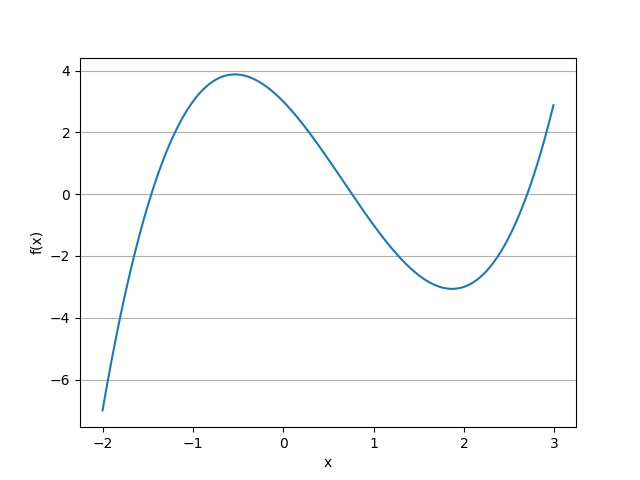
\includegraphics[width=65mm]{Figure_1.png}
	\end{figure}
\end{frame}

\begin{frame}
	\frametitle{解説}
	\framesubtitle{while文で繰り返し計算します。}
	\begin{itemize}
		\item 条件を満たすまで繰り返しを行うので、while文を使います。
		\item 絶対値を使うので、\#include\space\<math.h\>を忘れないようにしましょう。
	\end{itemize}
\end{frame}

\section{Lesson5}
\begin{frame}
	\frametitle{素因数分解}
	\begin{itembox}[l]{Q-5}
		変数に2以上の値を代入し、その数を素因数分解して得られる素数をすべて表示してください。\\
		最終的に変数に119028, 2146654199の2数を代入し出力してください。
	\end{itembox}
	\begin{block}{入力}
	\end{block}
	\begin{block}{出力例1}
		429 =\\
		3 ** 1\\
		11 ** 1\\
		13 ** 1\\
		49238 =\\
		2 ** 1\\
		7 ** 1\\
		3517 ** 1
	\end{block}
\end{frame}

\begin{frame}
	\begin{block}{出力例2}
		7502751 =\\
		3 ** 2\\
		47 ** 1\\
		17737 ** 1\\
		5104981 =\\
		7 ** 1\\
		17 ** 1\\
		42899 ** 1\\
	\end{block}
	\begin{block}{出力例3}
		9562 =\\
		2 ** 1\\
		7 ** 1\\
		683 ** 1\\
		515 =\\
		5 ** 1\\
		103 ** 1
	\end{block}
\end{frame}

\begin{frame}
	\frametitle{解説}
	\framesubtitle{while文を用いて、nが割り切れるまでiを増やすということをやります。}
	\begin{itemize}
		\item 再起処理を使えばコードが簡潔に書けるでしょう。
		\item 処理の速さを追及してみてください。
	\end{itemize}
\end{frame}

\section{Lesson6}
\begin{frame}
	\frametitle{ベクトルの内積}
	\begin{itembox}[l]{Q-6}
		大きさNのdouble型の配列a,bは、すべての要素に値が入った状態で与えられているとします。\\
		$$a = (1,2,3,\dots,N)$$
		$$b = (N, N-1, N-2,\dots,1)$$
		さらに、$N=1001$とし、その内積となす角を求めよ。
	\end{itembox}
\end{frame}
\end{document}
